% Options for packages loaded elsewhere
\PassOptionsToPackage{unicode}{hyperref}
\PassOptionsToPackage{hyphens}{url}
%
\documentclass[
]{article}
\usepackage{lmodern}
\usepackage{amssymb,amsmath}
\usepackage{ifxetex,ifluatex}
\ifnum 0\ifxetex 1\fi\ifluatex 1\fi=0 % if pdftex
  \usepackage[T1]{fontenc}
  \usepackage[utf8]{inputenc}
  \usepackage{textcomp} % provide euro and other symbols
\else % if luatex or xetex
  \usepackage{unicode-math}
  \defaultfontfeatures{Scale=MatchLowercase}
  \defaultfontfeatures[\rmfamily]{Ligatures=TeX,Scale=1}
\fi
% Use upquote if available, for straight quotes in verbatim environments
\IfFileExists{upquote.sty}{\usepackage{upquote}}{}
\IfFileExists{microtype.sty}{% use microtype if available
  \usepackage[]{microtype}
  \UseMicrotypeSet[protrusion]{basicmath} % disable protrusion for tt fonts
}{}
\makeatletter
\@ifundefined{KOMAClassName}{% if non-KOMA class
  \IfFileExists{parskip.sty}{%
    \usepackage{parskip}
  }{% else
    \setlength{\parindent}{0pt}
    \setlength{\parskip}{6pt plus 2pt minus 1pt}}
}{% if KOMA class
  \KOMAoptions{parskip=half}}
\makeatother
\usepackage{xcolor}
\IfFileExists{xurl.sty}{\usepackage{xurl}}{} % add URL line breaks if available
\IfFileExists{bookmark.sty}{\usepackage{bookmark}}{\usepackage{hyperref}}
\hypersetup{
  pdftitle={Homework 1},
  pdfauthor={David Elsheimer},
  hidelinks,
  pdfcreator={LaTeX via pandoc}}
\urlstyle{same} % disable monospaced font for URLs
\usepackage[margin=1in]{geometry}
\usepackage{color}
\usepackage{fancyvrb}
\newcommand{\VerbBar}{|}
\newcommand{\VERB}{\Verb[commandchars=\\\{\}]}
\DefineVerbatimEnvironment{Highlighting}{Verbatim}{commandchars=\\\{\}}
% Add ',fontsize=\small' for more characters per line
\usepackage{framed}
\definecolor{shadecolor}{RGB}{248,248,248}
\newenvironment{Shaded}{\begin{snugshade}}{\end{snugshade}}
\newcommand{\AlertTok}[1]{\textcolor[rgb]{0.94,0.16,0.16}{#1}}
\newcommand{\AnnotationTok}[1]{\textcolor[rgb]{0.56,0.35,0.01}{\textbf{\textit{#1}}}}
\newcommand{\AttributeTok}[1]{\textcolor[rgb]{0.77,0.63,0.00}{#1}}
\newcommand{\BaseNTok}[1]{\textcolor[rgb]{0.00,0.00,0.81}{#1}}
\newcommand{\BuiltInTok}[1]{#1}
\newcommand{\CharTok}[1]{\textcolor[rgb]{0.31,0.60,0.02}{#1}}
\newcommand{\CommentTok}[1]{\textcolor[rgb]{0.56,0.35,0.01}{\textit{#1}}}
\newcommand{\CommentVarTok}[1]{\textcolor[rgb]{0.56,0.35,0.01}{\textbf{\textit{#1}}}}
\newcommand{\ConstantTok}[1]{\textcolor[rgb]{0.00,0.00,0.00}{#1}}
\newcommand{\ControlFlowTok}[1]{\textcolor[rgb]{0.13,0.29,0.53}{\textbf{#1}}}
\newcommand{\DataTypeTok}[1]{\textcolor[rgb]{0.13,0.29,0.53}{#1}}
\newcommand{\DecValTok}[1]{\textcolor[rgb]{0.00,0.00,0.81}{#1}}
\newcommand{\DocumentationTok}[1]{\textcolor[rgb]{0.56,0.35,0.01}{\textbf{\textit{#1}}}}
\newcommand{\ErrorTok}[1]{\textcolor[rgb]{0.64,0.00,0.00}{\textbf{#1}}}
\newcommand{\ExtensionTok}[1]{#1}
\newcommand{\FloatTok}[1]{\textcolor[rgb]{0.00,0.00,0.81}{#1}}
\newcommand{\FunctionTok}[1]{\textcolor[rgb]{0.00,0.00,0.00}{#1}}
\newcommand{\ImportTok}[1]{#1}
\newcommand{\InformationTok}[1]{\textcolor[rgb]{0.56,0.35,0.01}{\textbf{\textit{#1}}}}
\newcommand{\KeywordTok}[1]{\textcolor[rgb]{0.13,0.29,0.53}{\textbf{#1}}}
\newcommand{\NormalTok}[1]{#1}
\newcommand{\OperatorTok}[1]{\textcolor[rgb]{0.81,0.36,0.00}{\textbf{#1}}}
\newcommand{\OtherTok}[1]{\textcolor[rgb]{0.56,0.35,0.01}{#1}}
\newcommand{\PreprocessorTok}[1]{\textcolor[rgb]{0.56,0.35,0.01}{\textit{#1}}}
\newcommand{\RegionMarkerTok}[1]{#1}
\newcommand{\SpecialCharTok}[1]{\textcolor[rgb]{0.00,0.00,0.00}{#1}}
\newcommand{\SpecialStringTok}[1]{\textcolor[rgb]{0.31,0.60,0.02}{#1}}
\newcommand{\StringTok}[1]{\textcolor[rgb]{0.31,0.60,0.02}{#1}}
\newcommand{\VariableTok}[1]{\textcolor[rgb]{0.00,0.00,0.00}{#1}}
\newcommand{\VerbatimStringTok}[1]{\textcolor[rgb]{0.31,0.60,0.02}{#1}}
\newcommand{\WarningTok}[1]{\textcolor[rgb]{0.56,0.35,0.01}{\textbf{\textit{#1}}}}
\usepackage{longtable,booktabs}
% Correct order of tables after \paragraph or \subparagraph
\usepackage{etoolbox}
\makeatletter
\patchcmd\longtable{\par}{\if@noskipsec\mbox{}\fi\par}{}{}
\makeatother
% Allow footnotes in longtable head/foot
\IfFileExists{footnotehyper.sty}{\usepackage{footnotehyper}}{\usepackage{footnote}}
\makesavenoteenv{longtable}
\usepackage{graphicx,grffile}
\makeatletter
\def\maxwidth{\ifdim\Gin@nat@width>\linewidth\linewidth\else\Gin@nat@width\fi}
\def\maxheight{\ifdim\Gin@nat@height>\textheight\textheight\else\Gin@nat@height\fi}
\makeatother
% Scale images if necessary, so that they will not overflow the page
% margins by default, and it is still possible to overwrite the defaults
% using explicit options in \includegraphics[width, height, ...]{}
\setkeys{Gin}{width=\maxwidth,height=\maxheight,keepaspectratio}
% Set default figure placement to htbp
\makeatletter
\def\fps@figure{htbp}
\makeatother
\setlength{\emergencystretch}{3em} % prevent overfull lines
\providecommand{\tightlist}{%
  \setlength{\itemsep}{0pt}\setlength{\parskip}{0pt}}
\setcounter{secnumdepth}{-\maxdimen} % remove section numbering
\usepackage{bm}
\usepackage{amsthm}
\newcommand{\Real}{\mathbb{R}}
\newcommand{\dom}{{\bf dom}\,}
\newcommand{\Tra}{^{\sf T}} % Transpose
\newcommand{\Inv}{^{-1}} % Inverse
\def\vec{\mathop{\rm vec}\nolimits}
\def\sweep{\mathop{\rm sweep}\nolimits}
\newcommand{\diag}{\mathop{\rm diag}\nolimits}
\newcommand{\tr}{\operatorname{tr}} % Trace
\newcommand{\epi}{\operatorname{epi}} % epigraph
\newcommand{\V}[1]{{\bm{\mathbf{\MakeLowercase{#1}}}}} % vector
\newcommand{\VE}[2]{\MakeLowercase{#1}_{#2}} % vector element
\newcommand{\Vn}[2]{\V{#1}^{(#2)}} % n-th vector
\newcommand{\Vtilde}[1]{{\bm{\tilde \mathbf{\MakeLowercase{#1}}}}} % vector
\newcommand{\Vhat}[1]{{\bm{\hat \mathbf{\MakeLowercase{#1}}}}} % vector
\newcommand{\VtildeE}[2]{\tilde{\MakeLowercase{#1}}_{#2}} % vector element
\newcommand{\M}[1]{{\bm{\mathbf{\MakeUppercase{#1}}}}} % matrix
\newcommand{\ME}[2]{\MakeLowercase{#1}_{#2}} % matrix element
\newcommand{\Mtilde}[1]{{\bm{\tilde \mathbf{\MakeUppercase{#1}}}}} % matrix
\newcommand{\Mhat}[1]{{\bm{\hat \mathbf{\MakeUppercase{#1}}}}} % matrix
\newcommand{\Mcheck}[1]{{\bm{\check \mathbf{\MakeUppercase{#1}}}}} % matrix
\newcommand{\Mbar}[1]{{\bm{\bar \mathbf{\MakeUppercase{#1}}}}} % matrix
\newcommand{\Mn}[2]{\M{#1}^{(#2)}} % n-th matrix

\title{Homework 1}
\author{David Elsheimer}
\date{Due @ 11:59pm on August 30, 2019}

\begin{document}
\maketitle

\textbf{Part 1.}

\begin{enumerate}
\def\labelenumi{\arabic{enumi}.}
\tightlist
\item
  Recall that the product property states:
\end{enumerate}

Let \(f_1 = \mathcal{O}(g_1)\) and \(f_2 = \mathcal{O}(g_2)\) Then
\(f_1 f_2 = \mathcal{O}(g_1g_2)\).

Prove the product property.

\textbf{Answer:}

\begin{proof}

Note by the definition of big $\mathcal{O}$-notation there exist $M_1, M_2, n_1, n_2$ such that $\lvert f_i(n)\rvert \leq M_i\lvert g_i(n)\rvert \ \forall n \geq n_i$.

Consider $M_{12} = max\{M_1,M_2\}, n_{12} = max\{n_1,n_2\}$. Further note  $\lvert f_i(n)\rvert \leq M_{1}M_2\lvert g_i(n)\rvert  \leq M_{12}\lvert g_i(n)\rvert \ \forall n \geq n_{12}$.

Before proceeding, note that $\lvert ab\rvert = \lvert a\rvert\lvert b\rvert$. This is easily shown by noting that $\lvert ab\rvert = \sqrt{(ab)^2} = \sqrt{a^2}\sqrt{b^2} = \lvert a\rvert\lvert b\rvert$.

$\lvert f_1(n)f_2(n)\rvert = \lvert f_1(n)\rvert\lvert f_2(n)\rvert\leq M_{1}M_2\lvert g_1(n)\rvert\lvert g_2(n)\rvert= M_{1}M_2\lvert g_1(n)g_2(n)\rvert$ for all $n \geq n_{12}$ and $\hat{M} = M_1M_2$.

Then $f_1 f_2 = \mathcal{O}(g_1g_2)$.

\end{proof}

\begin{enumerate}
\def\labelenumi{\arabic{enumi}.}
\setcounter{enumi}{1}
\tightlist
\item
  Let \({\bm{\mathbf{\MakeLowercase{v}}}} \in \mathbb{R}^n\) be a vector
  with unit Euclidean length,
  i.e.~\(\lVert {\bm{\mathbf{\MakeLowercase{v}}}} \rVert_2 = 1\). The
  Householder reflection of a point
  \({\bm{\mathbf{\MakeLowercase{x}}}} \in \mathbb{R}^n\) about the
  hyperplane that is orthogonal to \({\bm{\mathbf{\MakeLowercase{v}}}}\)
  is given by
\end{enumerate}

\[
h({\bm{\mathbf{\MakeLowercase{x}}}}; {\bm{\mathbf{\MakeLowercase{v}}}}) = {\bm{\mathbf{\MakeLowercase{x}}}} - 2 {\bm{\mathbf{\MakeLowercase{x}}}}^{\sf T}{\bm{\mathbf{\MakeLowercase{v}}}}{\bm{\mathbf{\MakeLowercase{v}}}}.
\] What is the fewest number of flops needed to compute the Householder
reflection
\(h({\bm{\mathbf{\MakeLowercase{x}}}}; {\bm{\mathbf{\MakeLowercase{v}}}})\)?

\textbf{Answer:}

To compute
\({\bm{\mathbf{\MakeLowercase{x}}}}^{\sf T}{\bm{\mathbf{\MakeLowercase{v}}}}\),
n + n-1 operations must be performed. This term is a scalar, so 2
\({\bm{\mathbf{\MakeLowercase{x}}}}^{\sf T}{\bm{\mathbf{\MakeLowercase{v}}}}\)
is computed in n+n = 2n flops. Thus 2
\({\bm{\mathbf{\MakeLowercase{x}}}}^{\sf T}{\bm{\mathbf{\MakeLowercase{v}}}}{\bm{\mathbf{\MakeLowercase{v}}}}\)
consists of 3n flops.

Therefore,
\({\bm{\mathbf{\MakeLowercase{x}}}} - 2{\bm{\mathbf{\MakeLowercase{x}}}}^{\sf T}{\bm{\mathbf{\MakeLowercase{v}}}}{\bm{\mathbf{\MakeLowercase{v}}}}\)
will consist of 4n flops. This is the fewest flops necessary to compute
the Householder reflection.

\textbf{Part 2.} Estimating areas under curves via Monte Carlo

You will use a Monte Carlo method to estimate areas under a curve,
specifically the Gaussian density function \[
\text{AUC}(a,b) = \int_a^b f(x)dx,
\] where \(f(x) = \frac{1}{\sqrt{2\pi}}e^{-\frac{x^2}{2}}\). We will
estimate the integral by throwing \(n\) darts at random onto a
rectangular canvas \([a,b] \times [0, 1/\sqrt{2\pi}]\) and counting the
fraction of darts that fall under the curve \(f\) on the canvas.

\includegraphics{mc_files/figure-latex/unnamed-chunk-1-1.pdf}

Let \(X_i\) and \(Y_i\) denote the \(x\) and \(y\) coordinates of the
\(i\)th dart. Suppose that \(X_i\) and \(Y_i\) are iid uniform\([a,b]\)
random variables and iid uniform\([0,\sqrt{2\pi}^{-1}]\) random
variables respectively. Let \(A_i\) denote the event that
\(Y_i \leq f(X_i)\). Then

\[
\text{AUC}(a,b) =  \frac{b-a}{\sqrt{2\pi}} P(A_1).
\]

We can estimate \(\text{AUC}(a,b)\) by plugging in an estimate of
\(P(A_1)\), namely \[
P(A_1) \approx \frac{1}{n}\sum_{i=1}^n I(A_i),
\] where \(I(A_i)\) is the indicator function of the event \(A_i\).

Please complete the following steps.

\textbf{Step 0:} Make an R package entitled ``your\_unityidST758''. My
unity id is ``ecchi'', so I would make a package entitled ecchiST758.
For the following functions, save them all in a file called
\texttt{homework1.R} and put this file in the R subdirectory of your
package.

\textbf{Step 1:} Write a function ``estimate\_auc'' that computes an
estimate of the area under the curve given a number of darts \texttt{n}.

\begin{Shaded}
\begin{Highlighting}[]
\CommentTok{#' Estimate auc}
\CommentTok{#' }
\CommentTok{#' \textbackslash{}code\{estimate_auc\} estimates the area under the curve via Monte Carlo}
\CommentTok{#' }
\CommentTok{#' @param n number of darts to throw}
\CommentTok{#' @param a left limit}
\CommentTok{#' @param b right limit}
\CommentTok{#' @export}
\NormalTok{estimate_auc <-}\StringTok{ }\ControlFlowTok{function}\NormalTok{(n, a, b) \{}
\NormalTok{((b}\OperatorTok{-}\NormalTok{a)}\OperatorTok{/}\NormalTok{(n}\OperatorTok{*}\KeywordTok{sqrt}\NormalTok{(}\DecValTok{2}\OperatorTok{*}\NormalTok{pi)))}\OperatorTok{*}\KeywordTok{sum}\NormalTok{(}\KeywordTok{exp}\NormalTok{(}\OperatorTok{-}\NormalTok{(}\KeywordTok{runif}\NormalTok{(n, a, b))}\OperatorTok{^}\DecValTok{2}\OperatorTok{/}\DecValTok{2}\NormalTok{)}\OperatorTok{/}\KeywordTok{sqrt}\NormalTok{(}\DecValTok{2}\OperatorTok{*}\NormalTok{pi) }
                           \OperatorTok{>=}\StringTok{ }\KeywordTok{runif}\NormalTok{(n, }\DecValTok{0}\NormalTok{, }\DecValTok{1}\OperatorTok{/}\KeywordTok{sqrt}\NormalTok{(}\DecValTok{2}\OperatorTok{*}\NormalTok{pi)))}
  
\NormalTok{\}}
\end{Highlighting}
\end{Shaded}

Your function should return an estimate of \(\text{AUC}(a,b)\).

\textbf{Step 2:} Plot your estimate of \(\text{AUC}(-1,1)\) as a
function of \(n\) for \(n = 10, 100, 1000, 10000\). Add a horizontal
line at the true value of the quantity you are trying to estimate,
namely \(y = \text{AUC}(-1,1)\).

\textbf{Answer:}

Note the true value of
\(AUC(-1,1)= \int_a^b \frac{1}{\sqrt{2\pi}}e^{-\frac{x^2}{2}}dx = \Phi(1) - \Phi(-1)\).
This can easily be calculated in R using \(\texttt{pnorm}\). The true
value is found to be 0.6826895.

A vector of values of the estimated AUC for
\(n \in \{10,100,1000,10000\}\) is provided below.

\begin{Shaded}
\begin{Highlighting}[]
\KeywordTok{library}\NormalTok{(ggplot2)}
\KeywordTok{set.seed}\NormalTok{(}\DecValTok{1002}\NormalTok{)}
\NormalTok{aucest<-}\StringTok{ }\KeywordTok{c}\NormalTok{(}\KeywordTok{estimate_auc}\NormalTok{(}\DecValTok{10}\NormalTok{,}\OperatorTok{-}\DecValTok{1}\NormalTok{,}\DecValTok{1}\NormalTok{),}
\KeywordTok{estimate_auc}\NormalTok{(}\FloatTok{1e2}\NormalTok{,}\OperatorTok{-}\DecValTok{1}\NormalTok{,}\DecValTok{1}\NormalTok{),}
\KeywordTok{estimate_auc}\NormalTok{(}\FloatTok{1e3}\NormalTok{,}\OperatorTok{-}\DecValTok{1}\NormalTok{,}\DecValTok{1}\NormalTok{),}
\KeywordTok{estimate_auc}\NormalTok{(}\FloatTok{1e4}\NormalTok{,}\OperatorTok{-}\DecValTok{1}\NormalTok{,}\DecValTok{1}\NormalTok{))}
\NormalTok{num<-}\StringTok{ }\KeywordTok{c}\NormalTok{(}\DecValTok{10}\NormalTok{,}\DecValTok{100}\NormalTok{,}\DecValTok{1000}\NormalTok{,}\DecValTok{10000}\NormalTok{)}
\NormalTok{plotdata<-}\StringTok{ }\KeywordTok{as.data.frame}\NormalTok{(}\KeywordTok{cbind}\NormalTok{(num,aucest))}
\NormalTok{plotdata}
\end{Highlighting}
\end{Shaded}

\begin{verbatim}
##     num    aucest
## 1    10 0.7180961
## 2   100 0.6861807
## 3  1000 0.6766061
## 4 10000 0.6832285
\end{verbatim}

\begin{Shaded}
\begin{Highlighting}[]
\KeywordTok{ggplot}\NormalTok{(}\DataTypeTok{data =}\NormalTok{ plotdata, }\KeywordTok{aes}\NormalTok{(}\DataTypeTok{x=}\NormalTok{num, }\DataTypeTok{y=}\NormalTok{aucest)) }\OperatorTok{+}\StringTok{ }\KeywordTok{geom_point}\NormalTok{()}\OperatorTok{+}
\StringTok{    }\KeywordTok{geom_line}\NormalTok{(}\DataTypeTok{linetype=}\StringTok{"dashed"}\NormalTok{)}\OperatorTok{+}\KeywordTok{geom_hline}\NormalTok{(}\DataTypeTok{yintercept=}\FloatTok{0.6826895}\NormalTok{, }\DataTypeTok{color =} \StringTok{"red"}\NormalTok{)}
\end{Highlighting}
\end{Shaded}

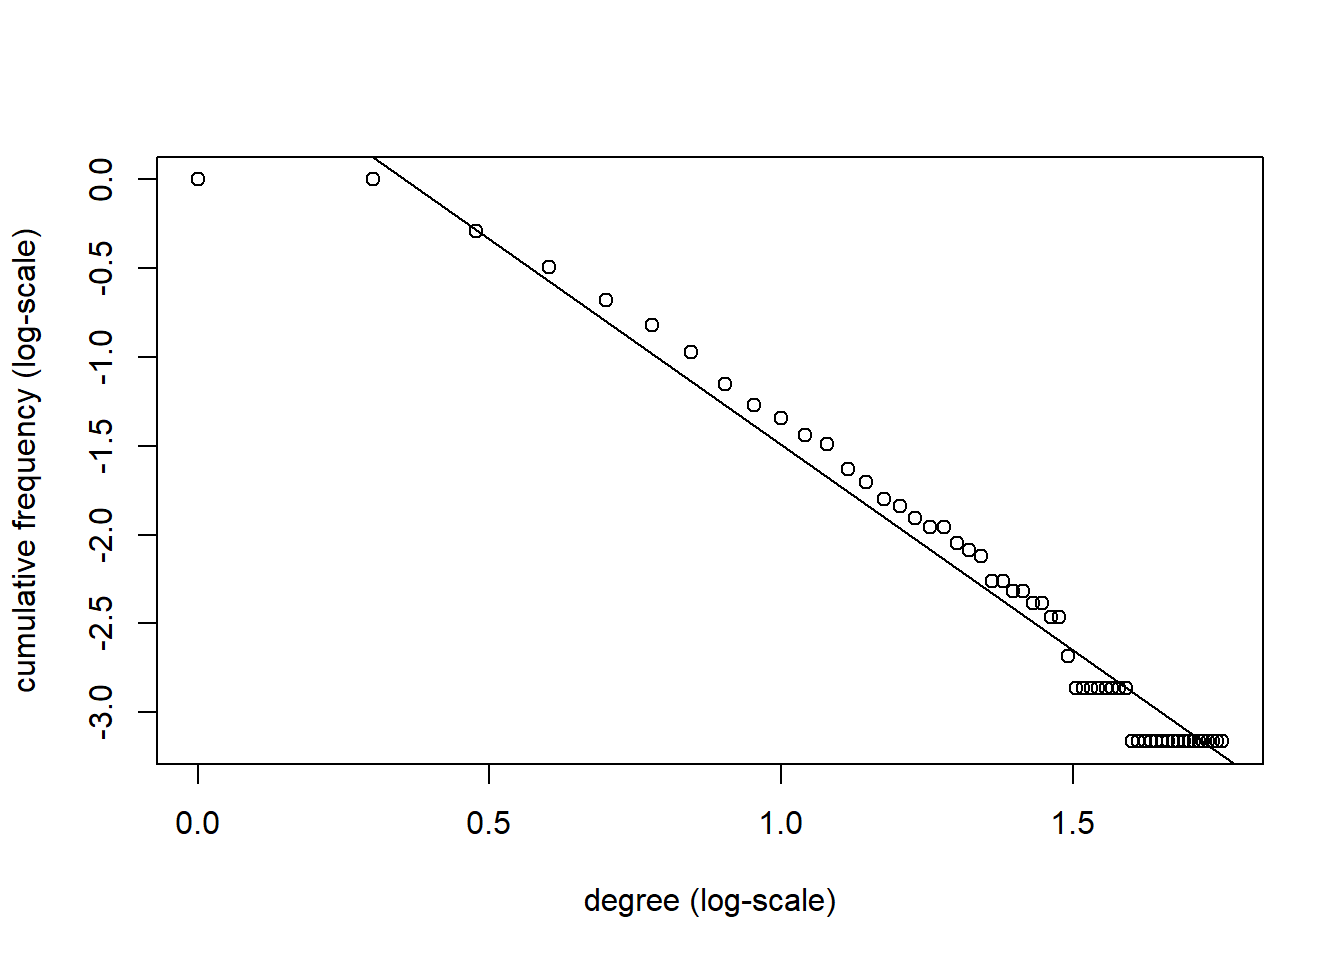
\includegraphics{mc_files/figure-latex/unnamed-chunk-3-1.pdf}

\textbf{Step 3:} Let \(Z_1, Z_2, ..., Z_n\) denote \(n\) independent
identically distributed random variables such that
\(\lvert Z_i \rvert \leq 1\) for \(i = 1, ..., n.\) Let \(\overline{Z}\)
denote the sample mean of \(Z_i\) and \(\mu\) denote the mean of
\(Z_1\). Recall that the Hoeffding bound tell us that

\[
P(\lvert \overline{Z} - \mu \rvert \geq t) \leq 2 \exp(-2 n t^2).
\]

Explain how you can use the Hoeffding bound to assess the correctness of
your function \texttt{estimate\_auc} and then write a small R script
below illustrating your evaluation. Suggestion: Consider redoing Step 2
using more information like multiple replicates, boxplots, and a
thoughtful application of the Hoeffding bound.

\textbf{Answer:}

Here, \(Z_i = I(Y_i \leq f(X_i))\). The \(Z_i\)'s are i.i.d., and
\(|Z_i| \leq 1\). Thus a Hoeffding bound is applicable here.
\(\bar{Z} = \frac{1}{n}\sum_{i=1}^nZ_i\). Here
\(E(Z_i) = P(Y_i \leq f(X_i))\). Due to \(Y_i\)'s being i.i.d, as well
as \(X_i\)'s being i.i.d., this can be further generalized as
\(P(Y\leq f(X))\).

Further note that \(P(Y\leq f(X)) = \frac{S}{c(b-a)}\), where \(a,b\)
are the bounds for \(X_i\), and \(c\) is the maximum density of
\(f(X)\), and \(S\) is the area under the curve.

Therefore, \(S = c(b-a)P(Y \leq f(X))\approx c(b-a)\bar{Z}\).

Applying the Hoeffding bound,
\(P(|c(b-a)\bar{Z} - c(b-a)P(Y\leq f(X))| \geq c(b-a)t)\leq 2\exp(-2n(c(b-a)t)^2)\).

Applying what has been demonstrated above, we can assess the correctness
of \texttt{estimate\_auc} using the following R script.

\begin{Shaded}
\begin{Highlighting}[]
\KeywordTok{library}\NormalTok{(tidyr)}
\KeywordTok{library}\NormalTok{(dplyr)}
\KeywordTok{library}\NormalTok{(forcats)}
\KeywordTok{set.seed}\NormalTok{(}\DecValTok{1002}\NormalTok{)}
\CommentTok{#Simulating estimates for different levels of n}
\CommentTok{#Creating boxplots at each level}
\NormalTok{num<-}\StringTok{ }\KeywordTok{c}\NormalTok{(}\DecValTok{10}\NormalTok{,}\DecValTok{50}\NormalTok{,}\DecValTok{100}\NormalTok{,}\DecValTok{500}\NormalTok{,}\DecValTok{1000}\NormalTok{,}\DecValTok{5000}\NormalTok{,}\DecValTok{10000}\NormalTok{)}
\NormalTok{auc_eval <-}\StringTok{ }\KeywordTok{replicate}\NormalTok{(}\KeywordTok{sapply}\NormalTok{(num,}\DataTypeTok{a=}\OperatorTok{-}\DecValTok{1}\NormalTok{,}\DataTypeTok{b=}\DecValTok{1}\NormalTok{, estimate_auc), }\DataTypeTok{n =}\DecValTok{1000}\NormalTok{)}
\NormalTok{auc_data <-}\StringTok{ }\KeywordTok{as.data.frame}\NormalTok{(}\KeywordTok{t}\NormalTok{(auc_eval)) }
\KeywordTok{colnames}\NormalTok{(auc_data) <-}\StringTok{ }\KeywordTok{c}\NormalTok{(}\StringTok{"10"}\NormalTok{, }\StringTok{"50"}\NormalTok{, }\StringTok{"100"}\NormalTok{, }\StringTok{"500"}\NormalTok{,}\StringTok{"1000"}\NormalTok{,}\StringTok{"5000"}\NormalTok{,}\StringTok{"10000"}\NormalTok{)}
\NormalTok{longauc <-}\StringTok{ }\KeywordTok{gather}\NormalTok{(auc_data,}\DataTypeTok{key=}\NormalTok{num)}
\NormalTok{longauc}\OperatorTok{$}\NormalTok{num<-}\KeywordTok{factor}\NormalTok{(longauc}\OperatorTok{$}\NormalTok{num, }\DataTypeTok{levels=}\KeywordTok{c}\NormalTok{(}\StringTok{"10"}\NormalTok{, }\StringTok{"50"}\NormalTok{, }\StringTok{"100"}\NormalTok{, }\StringTok{"500"}\NormalTok{,}\StringTok{"1000"}\NormalTok{,}\StringTok{"5000"}\NormalTok{,}\StringTok{"10000"}\NormalTok{))}
\KeywordTok{ggplot}\NormalTok{(}\DataTypeTok{data =}\NormalTok{ longauc, }\KeywordTok{aes}\NormalTok{(}\DataTypeTok{x=}\NormalTok{num, }\DataTypeTok{y=}\NormalTok{value)) }\OperatorTok{+}\StringTok{ }\KeywordTok{geom_boxplot}\NormalTok{() }\OperatorTok{+}
\StringTok{    }\KeywordTok{geom_hline}\NormalTok{(}\DataTypeTok{yintercept=}\FloatTok{0.6826895}\NormalTok{, }\DataTypeTok{color =} \StringTok{"red"}\NormalTok{) }\OperatorTok{+}\StringTok{ }
\StringTok{  }\KeywordTok{xlab}\NormalTok{(}\StringTok{"Number of darts thrown"}\NormalTok{) }\OperatorTok{+}\StringTok{ }
\StringTok{  }\KeywordTok{ylab}\NormalTok{(}\StringTok{"Area under curve via MC"}\NormalTok{)}
\end{Highlighting}
\end{Shaded}

\includegraphics{mc_files/figure-latex/unnamed-chunk-4-1.pdf}

\begin{Shaded}
\begin{Highlighting}[]
\CommentTok{#Checking that the probablities will be less than the bounds}
\NormalTok{probbound<-}\ControlFlowTok{function}\NormalTok{(n,t)\{}
  \DecValTok{2}\OperatorTok{*}\KeywordTok{exp}\NormalTok{(}\OperatorTok{-}\DecValTok{2}\OperatorTok{*}\NormalTok{n}\OperatorTok{*}\NormalTok{t}\OperatorTok{**}\DecValTok{2}\NormalTok{)}
\NormalTok{\}}
\NormalTok{true_y <-}\StringTok{ }\KeywordTok{pnorm}\NormalTok{(}\DecValTok{1}\NormalTok{)}\OperatorTok{-}\KeywordTok{pnorm}\NormalTok{(}\OperatorTok{-}\DecValTok{1}\NormalTok{)}
\NormalTok{longauc}\OperatorTok{$}\NormalTok{count_tol1 <-}\StringTok{ }\DecValTok{1}\OperatorTok{-}\StringTok{ }\KeywordTok{as.numeric}\NormalTok{(}\KeywordTok{between}\NormalTok{(longauc}\OperatorTok{$}\NormalTok{value,true_y}\FloatTok{-0.1}\NormalTok{,true_y}\FloatTok{+0.1}\NormalTok{))}
\NormalTok{longauc}\OperatorTok{$}\NormalTok{count_tol2 <-}\StringTok{ }\DecValTok{1}\OperatorTok{-}\KeywordTok{as.numeric}\NormalTok{(}\KeywordTok{between}\NormalTok{(longauc}\OperatorTok{$}\NormalTok{value,true_y}\FloatTok{-0.05}\NormalTok{,true_y}\FloatTok{+0.05}\NormalTok{))}
\NormalTok{longauc}\OperatorTok{$}\NormalTok{count_tol3 <-}\StringTok{ }\DecValTok{1}\OperatorTok{-}\KeywordTok{as.numeric}\NormalTok{(}\KeywordTok{between}\NormalTok{(longauc}\OperatorTok{$}\NormalTok{value,true_y}\FloatTok{-0.025}\NormalTok{,true_y}\FloatTok{+0.025}\NormalTok{))}
\NormalTok{probapprox <-}\StringTok{ }\NormalTok{longauc }\OperatorTok\StringTok{ }\KeywordTok{group_by}\NormalTok{(num)}\OperatorTok
\StringTok{  }\KeywordTok{summarise}\NormalTok{(}\KeywordTok{mean}\NormalTok{(count_tol1), }\KeywordTok{mean}\NormalTok{(count_tol2),}\KeywordTok{mean}\NormalTok{(count_tol3))}
\NormalTok{orderedprob <-}\StringTok{ }\NormalTok{probapprox}
\NormalTok{orderedprob}\OperatorTok{$}\NormalTok{probtol1 <-}\KeywordTok{sapply}\NormalTok{(num, }\DataTypeTok{t=}\FloatTok{0.1}\NormalTok{, probbound)}
\NormalTok{orderedprob}\OperatorTok{$}\NormalTok{probtol2 <-}\KeywordTok{sapply}\NormalTok{(num, }\DataTypeTok{t=}\FloatTok{0.05}\NormalTok{, probbound)}
\NormalTok{orderedprob}\OperatorTok{$}\NormalTok{probtol3 <-}\StringTok{ }\KeywordTok{sapply}\NormalTok{(num, }\DataTypeTok{t=}\FloatTok{0.025}\NormalTok{, probbound)}
\NormalTok{knitr}\OperatorTok{::}\KeywordTok{kable}\NormalTok{(orderedprob, }\DataTypeTok{col.names =} \KeywordTok{c}\NormalTok{(}\StringTok{"N"}\NormalTok{, }\StringTok{"$}\CharTok{\textbackslash{}\textbackslash{}}\StringTok{hat\{P\}(est}\CharTok{\textbackslash{}\textbackslash{}}\StringTok{notin$ tol-int 1)"}\NormalTok{,}
                           \StringTok{" $}\CharTok{\textbackslash{}\textbackslash{}}\StringTok{hat\{P\}(est}\CharTok{\textbackslash{}\textbackslash{}}\StringTok{notin$ tol-int 2)"}\NormalTok{, }
                           \StringTok{"$}\CharTok{\textbackslash{}\textbackslash{}}\StringTok{hat\{P\}(est}\CharTok{\textbackslash{}\textbackslash{}}\StringTok{notin$ tol-int 3)"}\NormalTok{, }
                           \StringTok{"Tol1 True prob"}\NormalTok{,}
                           \StringTok{"Tol2 True prob"}\NormalTok{,}
                           \StringTok{"Tol3 True prob"}\NormalTok{))}
\end{Highlighting}
\end{Shaded}

\begin{longtable}[]{@{}lrrrrrr@{}}
\toprule
\begin{minipage}[b]{0.03\columnwidth}\raggedright
N\strut
\end{minipage} & \begin{minipage}[b]{0.17\columnwidth}\raggedleft
\(\hat{P}(est\notin\) tol-int 1)\strut
\end{minipage} & \begin{minipage}[b]{0.18\columnwidth}\raggedleft
\(\hat{P}(est\notin\) tol-int 2)\strut
\end{minipage} & \begin{minipage}[b]{0.17\columnwidth}\raggedleft
\(\hat{P}(est\notin\) tol-int 3)\strut
\end{minipage} & \begin{minipage}[b]{0.08\columnwidth}\raggedleft
Tol1 True prob\strut
\end{minipage} & \begin{minipage}[b]{0.08\columnwidth}\raggedleft
Tol2 True prob\strut
\end{minipage} & \begin{minipage}[b]{0.08\columnwidth}\raggedleft
Tol3 True prob\strut
\end{minipage}\tabularnewline
\midrule
\endhead
\begin{minipage}[t]{0.03\columnwidth}\raggedright
10\strut
\end{minipage} & \begin{minipage}[t]{0.17\columnwidth}\raggedleft
0.367\strut
\end{minipage} & \begin{minipage}[t]{0.18\columnwidth}\raggedleft
0.367\strut
\end{minipage} & \begin{minipage}[t]{0.17\columnwidth}\raggedleft
1.000\strut
\end{minipage} & \begin{minipage}[t]{0.08\columnwidth}\raggedleft
1.6374615\strut
\end{minipage} & \begin{minipage}[t]{0.08\columnwidth}\raggedleft
1.9024588\strut
\end{minipage} & \begin{minipage}[t]{0.08\columnwidth}\raggedleft
1.9751556\strut
\end{minipage}\tabularnewline
\begin{minipage}[t]{0.03\columnwidth}\raggedright
50\strut
\end{minipage} & \begin{minipage}[t]{0.17\columnwidth}\raggedleft
0.013\strut
\end{minipage} & \begin{minipage}[t]{0.18\columnwidth}\raggedleft
0.236\strut
\end{minipage} & \begin{minipage}[t]{0.17\columnwidth}\raggedleft
0.523\strut
\end{minipage} & \begin{minipage}[t]{0.08\columnwidth}\raggedleft
0.7357589\strut
\end{minipage} & \begin{minipage}[t]{0.08\columnwidth}\raggedleft
1.5576016\strut
\end{minipage} & \begin{minipage}[t]{0.08\columnwidth}\raggedleft
1.8788261\strut
\end{minipage}\tabularnewline
\begin{minipage}[t]{0.03\columnwidth}\raggedright
100\strut
\end{minipage} & \begin{minipage}[t]{0.17\columnwidth}\raggedleft
0.002\strut
\end{minipage} & \begin{minipage}[t]{0.18\columnwidth}\raggedleft
0.093\strut
\end{minipage} & \begin{minipage}[t]{0.17\columnwidth}\raggedleft
0.386\strut
\end{minipage} & \begin{minipage}[t]{0.08\columnwidth}\raggedleft
0.2706706\strut
\end{minipage} & \begin{minipage}[t]{0.08\columnwidth}\raggedleft
1.2130613\strut
\end{minipage} & \begin{minipage}[t]{0.08\columnwidth}\raggedleft
1.7649938\strut
\end{minipage}\tabularnewline
\begin{minipage}[t]{0.03\columnwidth}\raggedright
500\strut
\end{minipage} & \begin{minipage}[t]{0.17\columnwidth}\raggedleft
0.000\strut
\end{minipage} & \begin{minipage}[t]{0.18\columnwidth}\raggedleft
0.000\strut
\end{minipage} & \begin{minipage}[t]{0.17\columnwidth}\raggedleft
0.043\strut
\end{minipage} & \begin{minipage}[t]{0.08\columnwidth}\raggedleft
0.0000908\strut
\end{minipage} & \begin{minipage}[t]{0.08\columnwidth}\raggedleft
0.1641700\strut
\end{minipage} & \begin{minipage}[t]{0.08\columnwidth}\raggedleft
1.0705229\strut
\end{minipage}\tabularnewline
\begin{minipage}[t]{0.03\columnwidth}\raggedright
1000\strut
\end{minipage} & \begin{minipage}[t]{0.17\columnwidth}\raggedleft
0.000\strut
\end{minipage} & \begin{minipage}[t]{0.18\columnwidth}\raggedleft
0.000\strut
\end{minipage} & \begin{minipage}[t]{0.17\columnwidth}\raggedleft
0.007\strut
\end{minipage} & \begin{minipage}[t]{0.08\columnwidth}\raggedleft
0.0000000\strut
\end{minipage} & \begin{minipage}[t]{0.08\columnwidth}\raggedleft
0.0134759\strut
\end{minipage} & \begin{minipage}[t]{0.08\columnwidth}\raggedleft
0.5730096\strut
\end{minipage}\tabularnewline
\begin{minipage}[t]{0.03\columnwidth}\raggedright
5000\strut
\end{minipage} & \begin{minipage}[t]{0.17\columnwidth}\raggedleft
0.000\strut
\end{minipage} & \begin{minipage}[t]{0.18\columnwidth}\raggedleft
0.000\strut
\end{minipage} & \begin{minipage}[t]{0.17\columnwidth}\raggedleft
0.000\strut
\end{minipage} & \begin{minipage}[t]{0.08\columnwidth}\raggedleft
0.0000000\strut
\end{minipage} & \begin{minipage}[t]{0.08\columnwidth}\raggedleft
0.0000000\strut
\end{minipage} & \begin{minipage}[t]{0.08\columnwidth}\raggedleft
0.0038609\strut
\end{minipage}\tabularnewline
\begin{minipage}[t]{0.03\columnwidth}\raggedright
10000\strut
\end{minipage} & \begin{minipage}[t]{0.17\columnwidth}\raggedleft
0.000\strut
\end{minipage} & \begin{minipage}[t]{0.18\columnwidth}\raggedleft
0.000\strut
\end{minipage} & \begin{minipage}[t]{0.17\columnwidth}\raggedleft
0.000\strut
\end{minipage} & \begin{minipage}[t]{0.08\columnwidth}\raggedleft
0.0000000\strut
\end{minipage} & \begin{minipage}[t]{0.08\columnwidth}\raggedleft
0.0000000\strut
\end{minipage} & \begin{minipage}[t]{0.08\columnwidth}\raggedleft
0.0000075\strut
\end{minipage}\tabularnewline
\bottomrule
\end{longtable}

As seen in the above simulation, for many randomly generated estimates,
as \(n\) increases, the accuracy of the estimate improves. This is clear
from how the boxplots get much smaller as \(n\) increases. The second
portion of the simulation is used to verify that the sample
probabilities of not being in the tolerance interval
\((\Phi(1) - \Phi(-1) \pm c(b-a))\) are smaller than their corresponding
Hoeffding bounds. This second portion of the simulation is performed for
tolerances 0.1, 0.05, and 0.025.

\textbf{Step 4:} Write a modified function, \texttt{estimate\_auc\_tol},
which returns an estimate of \(\text{AUC}(a,b)\) that is within a
specified tolerance \texttt{tol} with probability \texttt{p}, i.e.~your
output is within the true value of \(\text{AUC}(a,b)\) plus or minus
\texttt{tol} with probability \(p\).

\begin{Shaded}
\begin{Highlighting}[]
\CommentTok{#' Estimate auc}
\CommentTok{#' }
\CommentTok{#' \textbackslash{}code\{estimate_auc_tol\} estimates the area under the curve via Monte Carlo}
\CommentTok{#' }
\CommentTok{#' @param a left limit}
\CommentTok{#' @param b right limit}
\CommentTok{#' @param tol tolerance}
\CommentTok{#' @param p probability}
\CommentTok{#' @export}
\NormalTok{estimate_auc_tol <-}\StringTok{ }\ControlFlowTok{function}\NormalTok{(a, b, tol, p) \{}
\NormalTok{  n <-}\StringTok{ }\OperatorTok{-}\KeywordTok{log}\NormalTok{(p}\OperatorTok{/}\DecValTok{2}\NormalTok{)}\OperatorTok{/}\NormalTok{(}\DecValTok{2}\OperatorTok{*}\NormalTok{(tol)}\OperatorTok{^}\DecValTok{2}\NormalTok{)}
\NormalTok{  auctol <-}\StringTok{ }\NormalTok{((b}\OperatorTok{-}\NormalTok{a)}\OperatorTok{/}\NormalTok{(n}\OperatorTok{*}\KeywordTok{sqrt}\NormalTok{(}\DecValTok{2}\OperatorTok{*}\NormalTok{pi)))}\OperatorTok{*}\KeywordTok{sum}\NormalTok{(}\KeywordTok{exp}\NormalTok{(}\OperatorTok{-}\NormalTok{(}\KeywordTok{runif}\NormalTok{(n, a, b))}\OperatorTok{^}\DecValTok{2}\OperatorTok{/}\DecValTok{2}\NormalTok{)}\OperatorTok{/}\KeywordTok{sqrt}\NormalTok{(}\DecValTok{2}\OperatorTok{*}\NormalTok{pi) }
                           \OperatorTok{>=}\StringTok{ }\KeywordTok{runif}\NormalTok{(n, }\DecValTok{0}\NormalTok{, }\DecValTok{1}\OperatorTok{/}\KeywordTok{sqrt}\NormalTok{(}\DecValTok{2}\OperatorTok{*}\NormalTok{pi)))}
  \CommentTok{#Returning the estimated AUC with a specified tolerance, as well as the approximate n}
  \KeywordTok{return}\NormalTok{(}\KeywordTok{c}\NormalTok{(auctol, }\KeywordTok{ceiling}\NormalTok{(n)))}
\NormalTok{\}}
\end{Highlighting}
\end{Shaded}

As seen above, the primary change to this function is how \texttt{n} is
calculated for given \texttt{p}, \texttt{tol}. Examples of this function
being used are given below.

\begin{Shaded}
\begin{Highlighting}[]
\KeywordTok{estimate_auc_tol}\NormalTok{(}\OperatorTok{-}\DecValTok{1}\NormalTok{,}\DecValTok{1}\NormalTok{,}\FloatTok{0.5}\NormalTok{,}\FloatTok{0.5}\NormalTok{)}
\end{Highlighting}
\end{Shaded}

\begin{verbatim}
## [1] 0.287776 3.000000
\end{verbatim}

\begin{Shaded}
\begin{Highlighting}[]
\KeywordTok{estimate_auc_tol}\NormalTok{(}\OperatorTok{-}\DecValTok{1}\NormalTok{,}\DecValTok{1}\NormalTok{,}\DecValTok{1}\NormalTok{,}\FloatTok{0.1}\NormalTok{)}
\end{Highlighting}
\end{Shaded}

\begin{verbatim}
## [1] 0 2
\end{verbatim}

\begin{Shaded}
\begin{Highlighting}[]
\KeywordTok{estimate_auc_tol}\NormalTok{(}\OperatorTok{-}\DecValTok{1}\NormalTok{,}\DecValTok{1}\NormalTok{,}\FloatTok{0.05}\NormalTok{,}\FloatTok{0.05}\NormalTok{)}
\end{Highlighting}
\end{Shaded}

\begin{verbatim}
## [1]   0.6834908 738.0000000
\end{verbatim}

As the probability decreases, the estimate requires larger and larger n,
and the estimate trends towards the true AUC.

\textbf{Answer:}

The differences from the previous \texttt{estimate\_auc} function come
in the form of the tolerance and probability arguments. Another thing of
note is that here we do not provide the function with a number of
replicates, as it can be calculated using the tolerance and the
probability. As defined in problem 4, the tolerance is \(c(b-a)t\), and
the probability derived from the Hoeffding bound will be
\(2\exp(-2n(c(b-a))^2)\).

\textbf{Step 5:} Suppose instead of throwing darts at the canvas
\([a, b]\times[0,1/\sqrt{2\pi}]\), you decided to throw darts at the
canvas \([a, b]\times[0,c]\) for \(c \geq 1/\sqrt{2\pi}\). You still
count the fraction of darts that fall under the curve \(f\).
\textbf{Question 1:} Explain how you should modify your Monte Carlo
estimator of \(\text{AUC}(a,b)\) when you change the height of the
canvas. \textbf{Question 2:} What do you think will happen to the
quality of your estimator of \(\text{AUC}(a,b)\) as \(c\) increases?
\textbf{Question 3:} Design and run a simulation experiment that
illustrates the change in quality that you anticipate. Use a modified
version of your `estimate\_auc' function called
`estimate\_auc\_modified'.

\begin{Shaded}
\begin{Highlighting}[]
\CommentTok{#' Estimate auc modified}
\CommentTok{#' }
\CommentTok{#' \textbackslash{}code\{estimate_auc_modified\} estimates the area under the curve via Monte Carlo}
\CommentTok{#' }
\CommentTok{#' @param n number of darts to throw}
\CommentTok{#' @param a left limit}
\CommentTok{#' @param b right limit}
\CommentTok{#' @param c canvas dimension variable}
\CommentTok{#' @export}
\NormalTok{estimate_auc_modified <-}\StringTok{ }\ControlFlowTok{function}\NormalTok{(n, a, b, }\DataTypeTok{c=}\DecValTok{1}\OperatorTok{/}\KeywordTok{sqrt}\NormalTok{(}\DecValTok{2}\OperatorTok{*}\NormalTok{pi)) \{}
\ControlFlowTok{if}\NormalTok{(c}\OperatorTok{<}\StringTok{ }\DecValTok{1}\OperatorTok{/}\KeywordTok{sqrt}\NormalTok{(}\DecValTok{2}\OperatorTok{*}\NormalTok{pi)) }\KeywordTok{stop}\NormalTok{(}\StringTok{"Canvas height too low"}\NormalTok{)}
  
\NormalTok{  ((b}\OperatorTok{-}\NormalTok{a)}\OperatorTok{/}\NormalTok{(n}\OperatorTok{*}\KeywordTok{sqrt}\NormalTok{(}\DecValTok{2}\OperatorTok{*}\NormalTok{pi)))}\OperatorTok{*}\KeywordTok{sum}\NormalTok{(}\KeywordTok{exp}\NormalTok{(}\OperatorTok{-}\NormalTok{(}\KeywordTok{runif}\NormalTok{(n, a, b))}\OperatorTok{^}\DecValTok{2}\OperatorTok{/}\DecValTok{2}\NormalTok{)}\OperatorTok{/}\KeywordTok{sqrt}\NormalTok{(}\DecValTok{2}\OperatorTok{*}\NormalTok{pi) }
                           \OperatorTok{>=}\StringTok{ }\KeywordTok{runif}\NormalTok{(n, }\DecValTok{0}\NormalTok{, c))}
  
\NormalTok{\}}
\end{Highlighting}
\end{Shaded}

Your function should return an estimate of \(\text{AUC}(a,b)\) and
should return an error if \(c < 1/\sqrt{2\pi}\).

\textbf{Answer:}

The modification is simple. The change here is that \(Y \sim U(0,c)\).
This will change the estimator with respect to how the height of the
canvas changes. Notice that for fixed \(a,b\) where \(b>a\), X is
bounded between
\((\frac{1}{\sqrt{2\pi}}e^{-b^2/2}, \frac{1}{\sqrt{2\pi}})\). As c
increases, \(P(A_1) \approx \frac{1}{n}\sum_{i=1}^nI(A_i)\) will
decrease because it will become increasingly likely that there will be
values of \(y_i>f(x_i)\). Thus the quality of the estimator will
decrease for greater values of \(c\). This can be coded fairly easily,
as seen above and in the dbelsheiST758 package. A condition is included
to return errors for canvases shorter than the minimum height.

\begin{Shaded}
\begin{Highlighting}[]
\KeywordTok{set.seed}\NormalTok{(}\DecValTok{1002}\NormalTok{)}
\CommentTok{#demonstrating the behavior}
\KeywordTok{estimate_auc_modified}\NormalTok{(}\DecValTok{10}\NormalTok{,}\OperatorTok{-}\DecValTok{1}\NormalTok{,}\DecValTok{1}\NormalTok{, }\DataTypeTok{c=} \FloatTok{.1}\NormalTok{)}
\end{Highlighting}
\end{Shaded}

\begin{verbatim}
## Error in estimate_auc_modified(10, -1, 1, c = 0.1): Canvas height too low
\end{verbatim}

\begin{Shaded}
\begin{Highlighting}[]
\KeywordTok{estimate_auc_modified}\NormalTok{(}\DecValTok{10}\NormalTok{,}\OperatorTok{-}\DecValTok{1}\NormalTok{,}\DecValTok{1}\NormalTok{)}
\end{Highlighting}
\end{Shaded}

\begin{verbatim}
## [1] 0.7180961
\end{verbatim}

\begin{Shaded}
\begin{Highlighting}[]
\KeywordTok{estimate_auc_modified}\NormalTok{(}\DecValTok{10}\NormalTok{,}\OperatorTok{-}\DecValTok{1}\NormalTok{,}\DecValTok{1}\NormalTok{, }\DataTypeTok{c=} \DecValTok{3}\NormalTok{)}
\end{Highlighting}
\end{Shaded}

\begin{verbatim}
## [1] 0.07978846
\end{verbatim}

\begin{Shaded}
\begin{Highlighting}[]
\KeywordTok{estimate_auc_modified}\NormalTok{(}\DecValTok{10}\NormalTok{,}\OperatorTok{-}\DecValTok{1}\NormalTok{,}\DecValTok{1}\NormalTok{, }\DataTypeTok{c=} \DecValTok{4}\NormalTok{)}
\end{Highlighting}
\end{Shaded}

\begin{verbatim}
## [1] 0
\end{verbatim}

\end{document}
